% Image wrapper: PDF table structure was not recoverable automatically.
% Requires \usepackage{graphicx}. Replace the image with tabular cells when editable text is needed.
% Caption: Table 1 and 2 present the ∆PSNR in CBR mode and CQP mode.The results show that our method performs best in both two modes for average ∆PSNR. Comparing to the CBREN which is specially designed for CBR Videos quality enhancement,ourmethodbeatitby0.07dBand0.13dB(upto20\%)inCBRmode.Meanwhile,ourHFURalso achieve the best performance on all test sequences and beat the second best BasicVSR++ by 0.13dB and 0.17dB in CQP mode.We also provide the visualized results of compared methods in Fig. 5.The compressed patches suffer from various compression artifacts including blocking (in BasketballPass), color bleeding (in PartyScene), and ringing (in RaceHorses).Existing methods fail to recognize the artifacts and cannot appropriately suppress the artifacts (e.g., wrong texture on the wall, ringing effect in the horses) or restore the missing details (e.g., border between the clothes and the background).Thanks to the powerful frequency-domain information reconstruction, our HFUR could accurately recover the details or textures through the frequency domain and produce more visual pleased results.Further experimental and visualized results are available in the Supplementary Material.
\begin{tabular}{c}
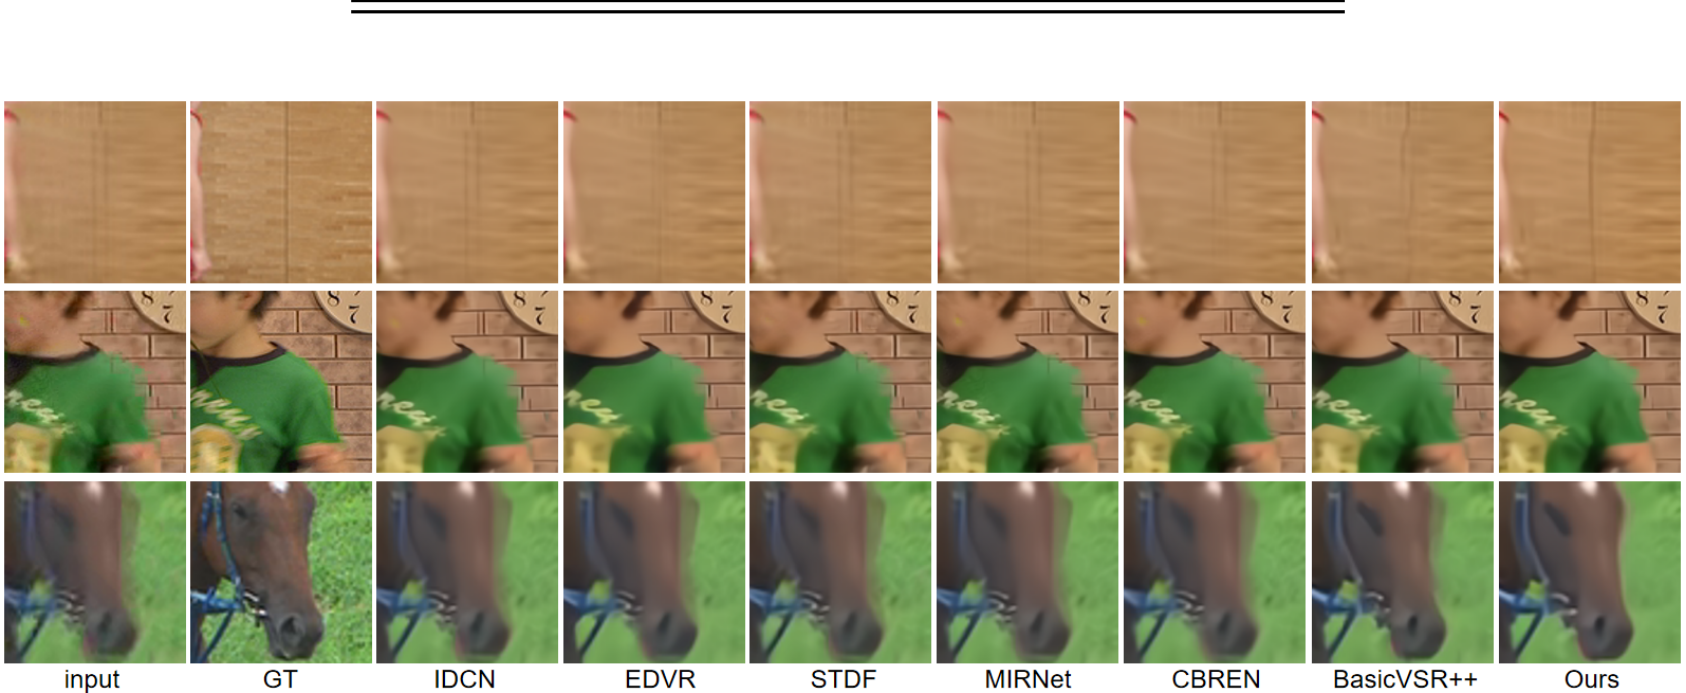
\includegraphics[width=\linewidth]{../original/Table1_p008.png}
\end{tabular}
